\chapter{The Cosmic Microwave Background}
The goal of this chapter will be to understand a little bit more quantitatively why the Cosmic Microwave background is so important in the study of cosmology; in particular we want to understand how one can extract meaningful information from the sky temperature measurements of the CMB. As we have seen, the CMB is the radiation leftover from the bigbang, which originated at the epoch of recombination, when the universe became charge neutral and the photons decoupled from matter, free streaming toward us, when we measure them. We measure the temperature of this radiation (in the sense pointed out in Chapter \ref{chp7}) to be $T_{CMB}=2.78$K (see Figure \ref{cmbspectral} for reference). As of now, we have approximated this radiation as uniform all over the sky; in reality, as previously announced, the spatial temperature profile of the CMB is not uniform, but contains very tiny fluctuations of relative order $\frac{\delta T}{T}\approx 10^{-5}$, as you can see in Figure \ref{cmbwmap}, which is a full sky CMB 
map taken by the WMAP satellite 
\begin{figure}
\begin{center}
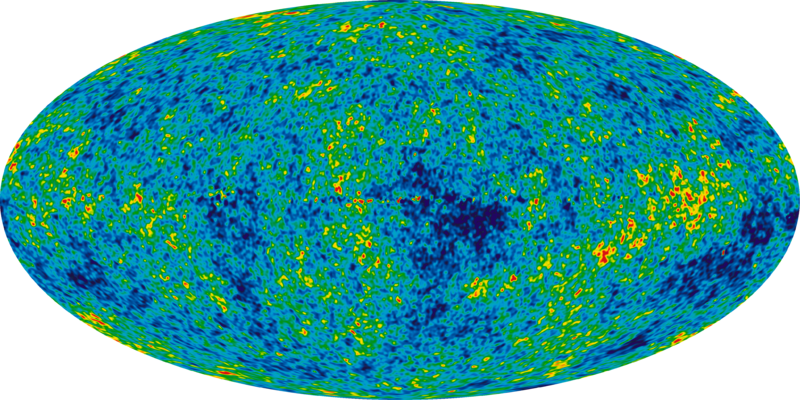
\includegraphics[scale=0.5]{CMB/wmap}
\label{}
\end{center}
\caption{A full sky map of the Cosmic Microwave Background, from the experiment WMAP: the fluctuations in temperature from red to blue spots have a relative magnitude $\delta T/T\sim 10^{-5}$.  Credit for the image \url{http://apod.nasa.gov/apod/ap030212.html}}
\label{cmbwmap}
\end{figure}
What this map really represents is a (very accurate) snapshot on how the universe was at the time of recombination (i.e. when it was only $t_{rec}\sim 300,000$\,yr old), capturing all the inhomogeneities that were present at that time, and that we believe originated all the collapsed structures (star, galaxies,etc...) that we see today. In this chapter we want to understand better how we can extract cosmological information from the spatial arrangement and size of these inhomogeneities, and what are the physical mechanism that originated them. Before doing this, however, we need to master some useful mathematical tools for analyzing scale dependent variations, namely the basics of Fourier analysis. 

\section{How do we describe inhomogeneities quantitatively?}
\label{fouriersection}
In physics there are plenty of examples where we have to deal with quantities that are non uniform and vary in space; you can think about the temperature profile of a conducting rod (1 dimensional variation), the height of the water ripples on a lake (2 dimensional variations) or the density profile of a gas cloud in the interstellar medium (3 dimensional variation). In the following, we will give a brief summary on how to analyze these different kinds of inhomogeneities. 
\subsection{One dimensional inhomogeneities}
Think about a simple example os outlined before we have a long metal cable fixed at two points; suppose that some physical mechanism acting on this rod makes it oscillate, and each point $x$ on the cable is displaced from its equilibrium position by an amount $y=f(x)$ (at fixed time) with $f$ some function of $x$. Consider the example where $f$ describes a simple harmonic wave, as in Figure \ref{fourier1d} (think of all the lengths expressed in cm)
\begin{figure}
\begin{center}
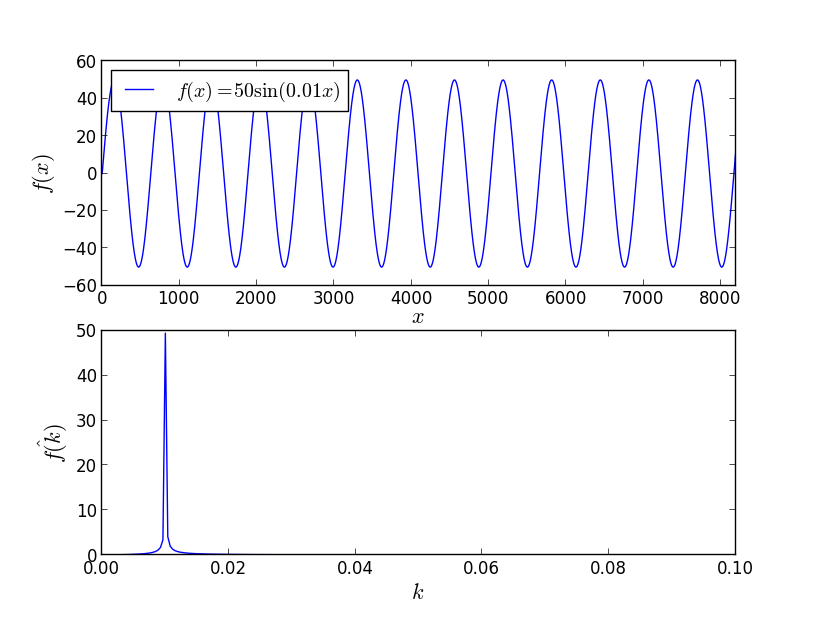
\includegraphics[scale=0.7]{Fourier/1component.png}
\label{}
\end{center}
\caption{The profile of an harmonic wave traveling on a metal cable; the meaningful variations in the cable profile occur on a spatial scale $\lambda=\frac{2\pi}{k}=\frac{2\pi}{0.01}$; the Fourier transform $\hat{f}(k)$ captures this feature}
\label{fourier1d}
\end{figure}
We can see that the inhomogeneities in the cable profile occur on a spatial scale of $\lambda=\frac{2\pi}{0.01}\,\mathrm{cm}\approx 600\,\mathrm{cm}$; if we look on scale lengths much smaller than $600$\,cm we won't notice that the cable profile is inhomogeneous. We will see the inhomogeneities only when we look at scale comparables with $\lambda$; this is precisely what the bottom panel of Figure \ref{fourier1d} tells us: the \textit{Fourier transform} $\hat{f}(k)$ is a function that can be uniquely calculated from the original function $f$ and tells us how much information of $f$ is stored in a scale $\lambda=\frac{2\pi}{k}$. We see that, in this case, all the information is stored in a unique scale $\lambda$ corresponding to a \textit{wavenumber} $k=0.01\mathrm{cm}^{-1}$. The way this Fourier transform is calculated, is by \textit{matching} our original function $f$ with a \textit{template} that contains information in a single scale only (in this case a sine function $\sin{kx}$) 
\begin{equation}
\label{trasf1d}
\hat{f}(k)=\int_0^Lf(x)\sin{(kx)}dx
\end{equation}
When $\hat{f}(k)=0$, it means that our function $f(x)$ doesn't contain any information on the particular spatial scale $\lambda=\frac{2\pi}{k}$; to illustrate the usefulness of this way of analyzing inhomogeneities, consider the following two examples outlined in Figure \ref{fourier23d}
\begin{figure}
\begin{center}
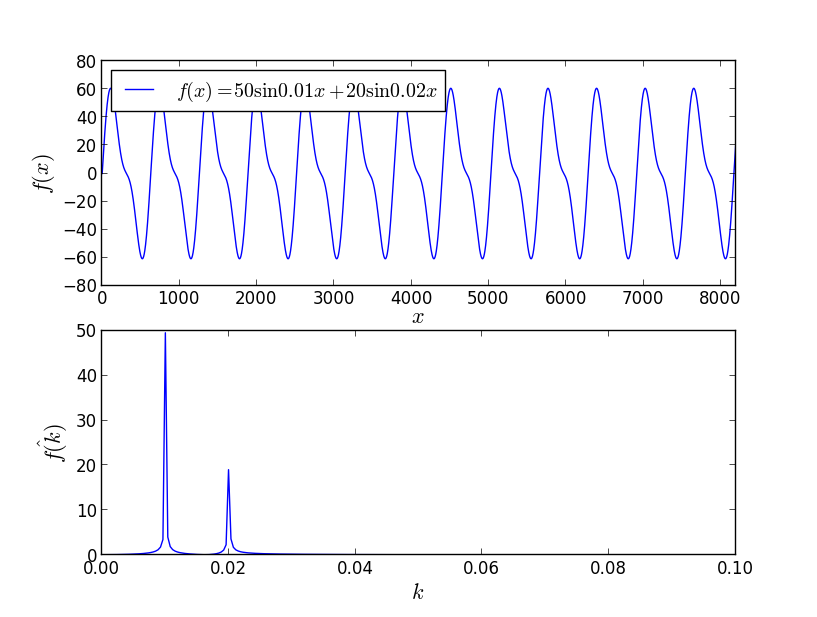
\includegraphics[scale=0.4]{Fourier/2component.png}
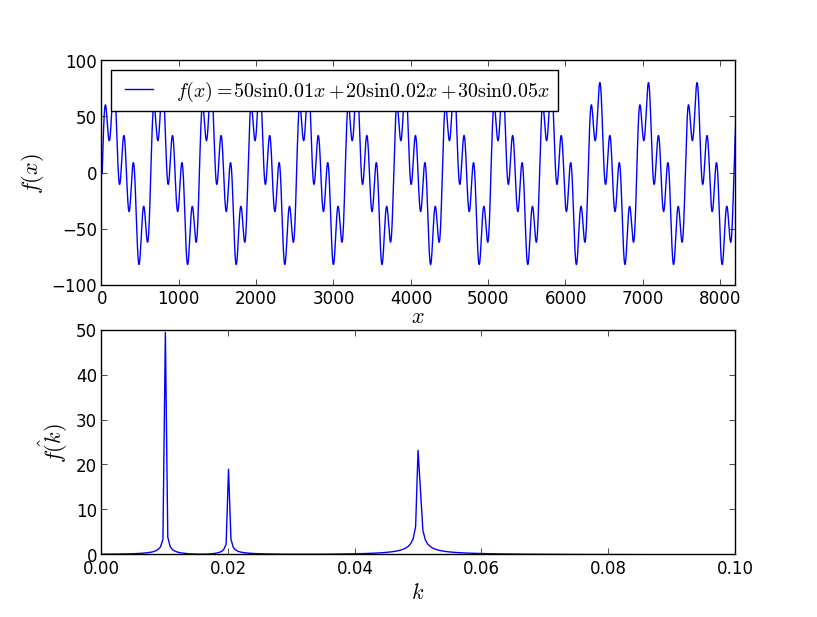
\includegraphics[scale=0.4]{Fourier/3component.png}
\label{}
\end{center}
\caption{Examples of functions whose inhomogeneities contain information on multiple length scales, namely 2(left panel) or 3(right panel)}
\label{fourier23d}
\end{figure}
We immediately see that, even if the cable profiles become messy, this Fourier analysis trick tells us immediately where (in which spatial scales) the relevant information is stored. Fourier analysis can also be quite useful in extracting a signal from a noisy background; consider for example Figure \ref{gaussnoise}
\begin{figure}
\begin{center}
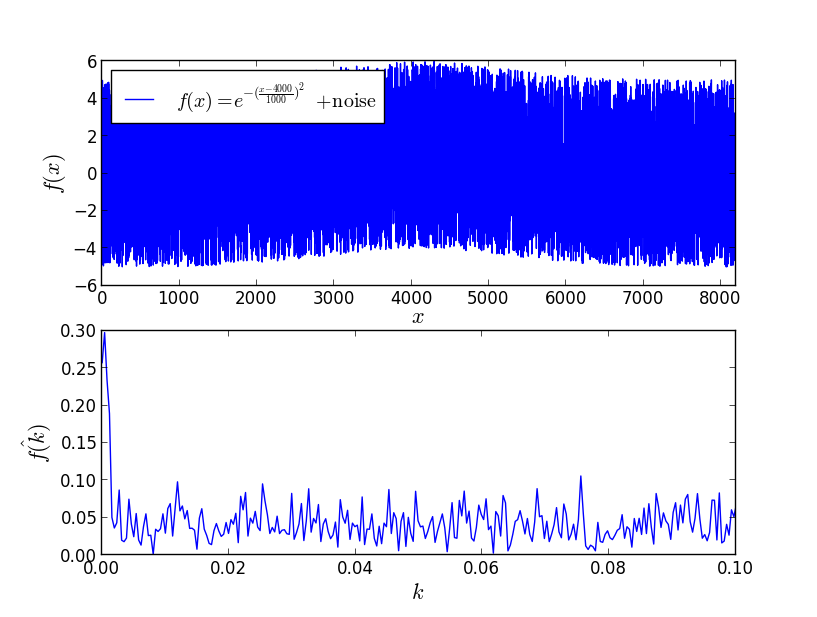
\includegraphics[scale=0.6]{Fourier/gauss+noise.png}
\label{}
\end{center}
\caption{A gaussian peak $f(x)\propto e^{-(x-\mu)^2/2\sigma^2}$ contains information on a length scale $\sigma \gg \lambda_{noise}$, and hence a Fourier analysis is able to separate the signal information from the noise background, which acts on much smaller length scales }
\label{gaussnoise}
\end{figure}
In this case the signal (a gaussian peak) contains information on a scale which is much bigger than the typical scale of the noise; we clearly see this feature in the Fourier transform in Figure \ref{gaussnoise}, which peaks at low $k$ can distinguish clearly the signal contribution from the noise one. We want to extend this concept of one dimensional Fourier analysis to 2d inhomogeneities, with our goal to understand 2 dimensional CMB maps in mind. 
\subsection{Two dimensional inhomogeneities}
\label{2dsection}
In this section, we wish to extends all the concepts of Fourier analysis presented before, but applied to two dimensional systems (for example a two dimensional temperature map of the CMB sky); what we will need is find suitable templates that correspond to a particular spatial scales, and a prescription similar to equation (\ref{trasf1d}) to compare them with the non homogeneous field we wish to analyze. If our 2 dimensional space were to be infinite and flat, we would use templates in the form $\tau_{k_x,k_y}=\sin{ (k_x x)}\sin{(k_y y)}$ in analogy to what we have already done; it turns out however that in the case of the CMB our field of view is neither infinite nor flat. In particular it is the inner surface of a sphere, which we have already seen we can describe in terms of two angular coordinates $(\theta,\phi)$ as in Figure \ref{coordinates}, fixing the radius to $r=1$. What our current experiments do is measuring the temperature profile on sky $T(\mathbf{\hat{n}})=T(\theta,\phi)$ varying the 
direction of observation $\mathbf{\hat{n}}=(\sin \theta \cos \phi,\sin \theta \sin \phi,\cos \theta)$; it turns out that for describing the temperature field $T(\mathbf{\hat{n}})$ the most suitable templates, which encode the scale which we want to extract the information about, are some special functions called \textit{spherical harmonics}. These functions are labelled each by a couple of integer numbers $(l,m)$, where $l=0,1,2,....$ and $-l\leq m \leq l$; to understand to which angular scale each template corresponds, we have to know the fact that
\begin{equation}
Y_{ll}(\theta,\phi)\propto \cos^l\theta \sin{(l\phi)}
\end{equation}
which, if you think about it a little bit, exibits significant variations on an angular scale $\delta \theta \approx \delta\phi \approx \pi/l$. We don't want to go into the details of these spherical harmonics too much, but it can be shown that a similar behaviour holds also for the spherical harmonics with $m\neq l$; for the sake of understanding all we need is know that a spherical harmonic $Y_{lm}$ can serve us as a template to extract information from a sky temperature map $T(\mathbf{\hat{n}}$) on an angular scale $\pi/l=180^\circ/l$. In Figure \ref{sphharmonics} are some examples of sky temperature maps built with only one template (i.e. that contain information on only one angular scale, analogously to Figure \ref{fourier1d}). 
\begin{figure}
\begin{center}
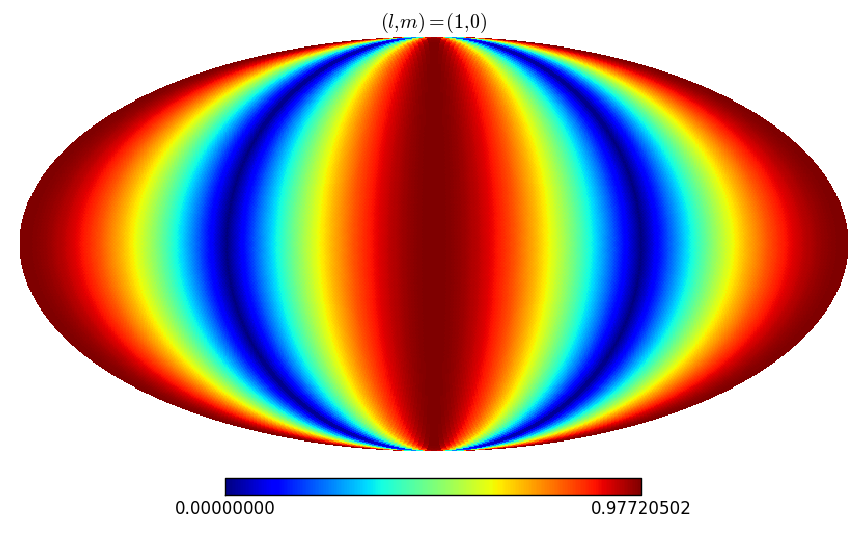
\includegraphics[scale=0.3]{Fourier/(1,0).png}
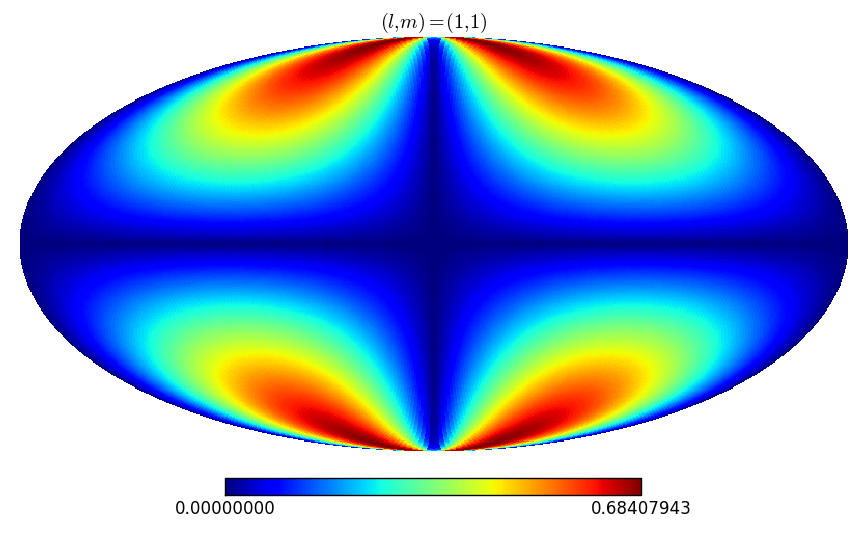
\includegraphics[scale=0.3]{Fourier/(1,1).png}
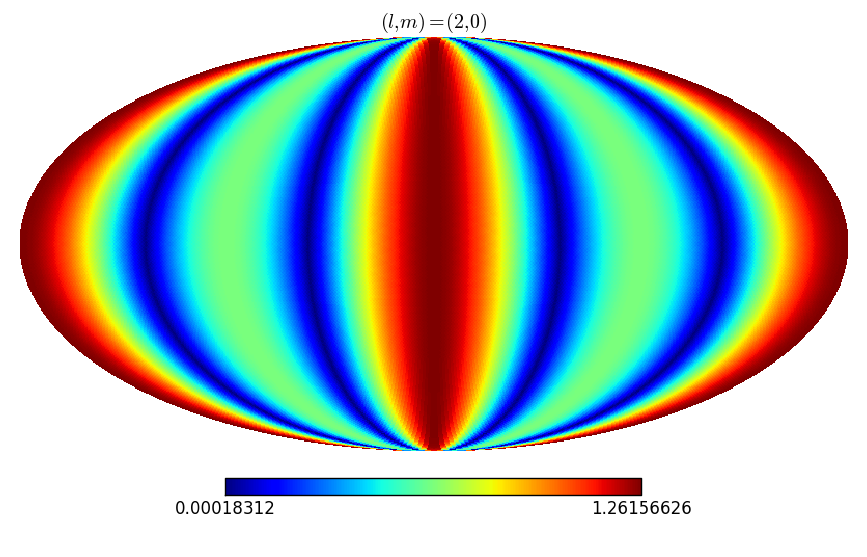
\includegraphics[scale=0.3]{Fourier/(2,0).png}
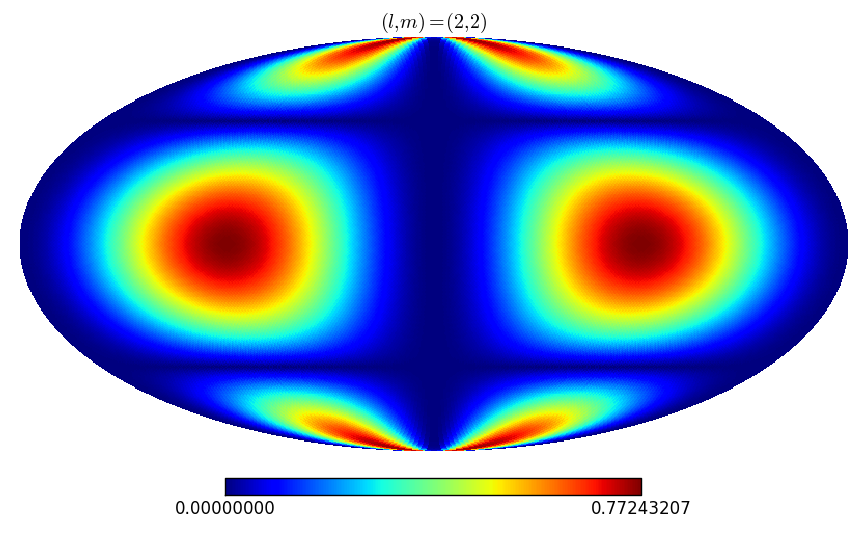
\includegraphics[scale=0.3]{Fourier/(2,2).png}
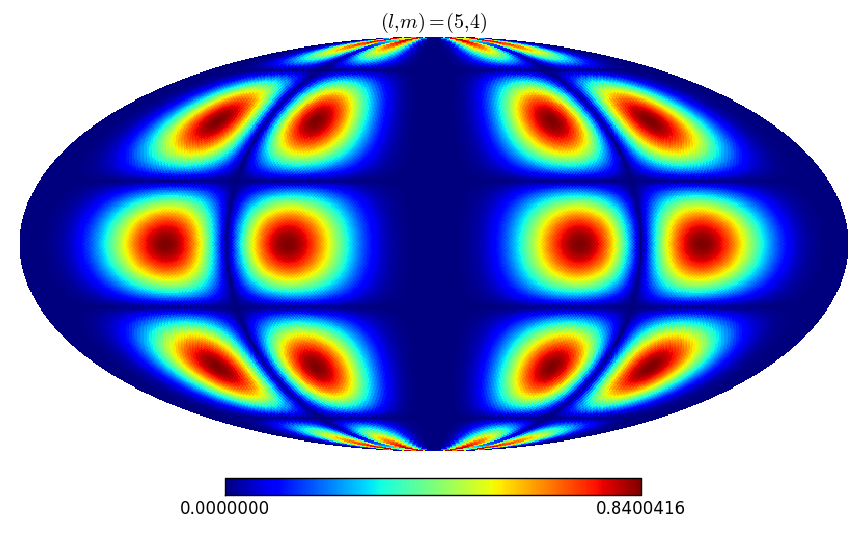
\includegraphics[scale=0.3]{Fourier/(5,4).png}
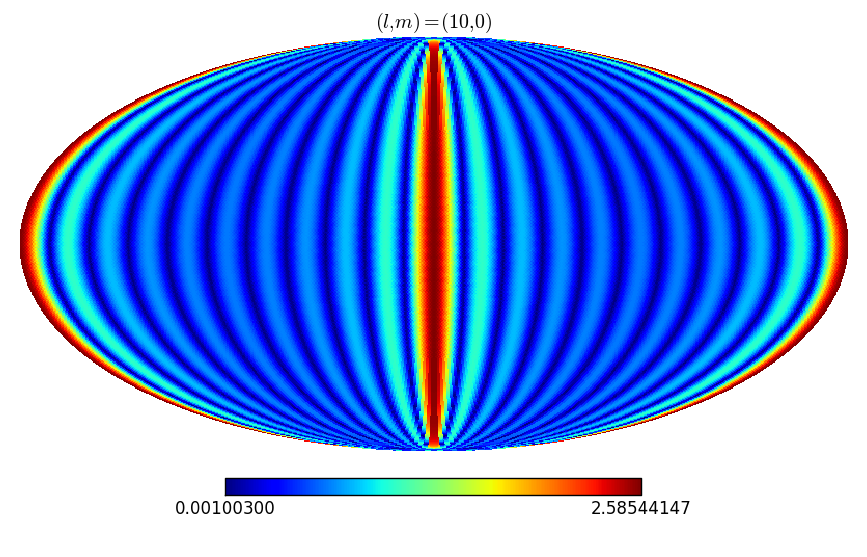
\includegraphics[scale=0.3]{Fourier/(10,0).png}
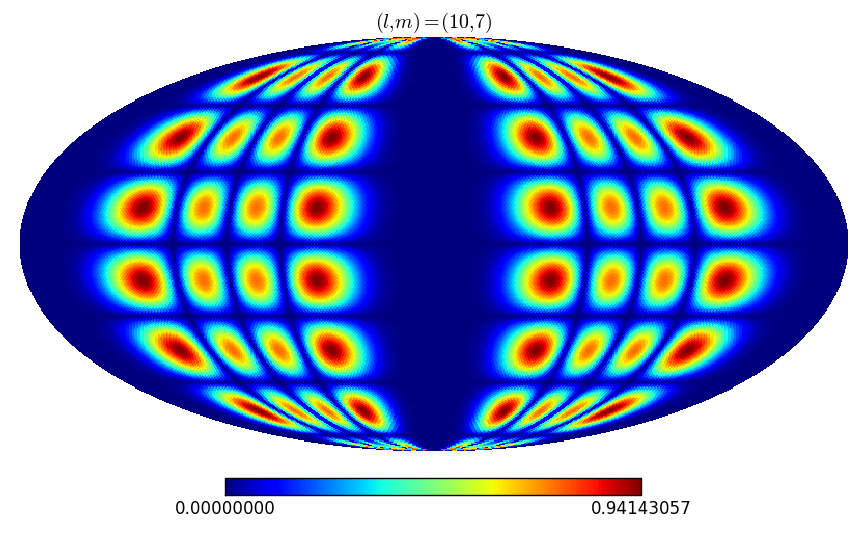
\includegraphics[scale=0.3]{Fourier/(10,7).png}
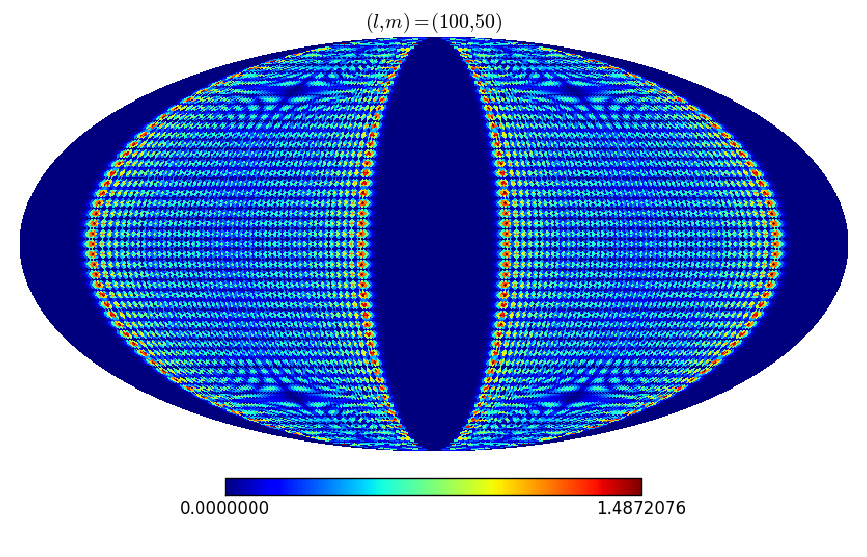
\includegraphics[scale=0.3]{Fourier/(100,50).png}
\end{center}
\caption{Whole sky maps of $Y_{l,m}(\theta,\phi)+Y_{l,-m}(\theta ,\phi)$ in mollweide projection for $(l,m)=(1,0),(1,1),(2,0),(2,2),(5,4),(10,0),(10,7),(100,50)$ 
from left to right, top to bottom}
\label{sphharmonics}
\end{figure}
As you can see increasing $l$ decreases the angular scale of the template, while changing $m$ has to do with the rotational symmetry of the arrangement: $m=0$ means the template is symmetric for rotations along the horizontal axis, which is $\mathbf{\hat{z}}$ in mollweide projection, while $m\neq 0$ introduces a periodic structure in $\phi$ with period $2\pi/m$. One can think of a sky map that contains information on multiple scales, in analogy with Figure \ref{fourier23d}, and think and about an example like Figure \ref{superp}
\begin{figure}
\begin{center}
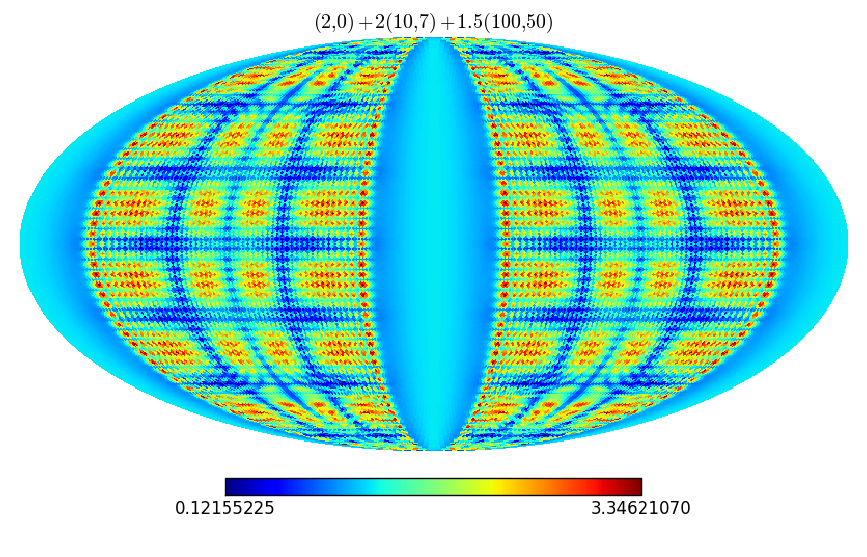
\includegraphics[scale=0.6]{Fourier/superp.png}
\label{}
\end{center}
\caption{A whole sky map that contains relevant information on three different angular scales, and receives contributions from three templates, $l=2,l=10$ and $l=100$, with relative weights 1,2,1.5}
\label{superp}
\end{figure}
A real world CMB map however won't be so easy to describe, because it will contain information on \textit{all} angular scales (this last example contains information only on three different angular scales); depending on the angular resolution of our experiment, call it $\delta \theta$, we will be able to probe the CMB sky only up to a maximum $l_{max}\sim 180^\circ/\delta \theta$. Depending on how big is the $l_{max}$ we are able to probe, our real CMB sky can look quite different when we image it, as you can see in Figure \ref{simcmbsky}. We will explain this better in the following paragraph. 
\begin{figure}
\begin{center}
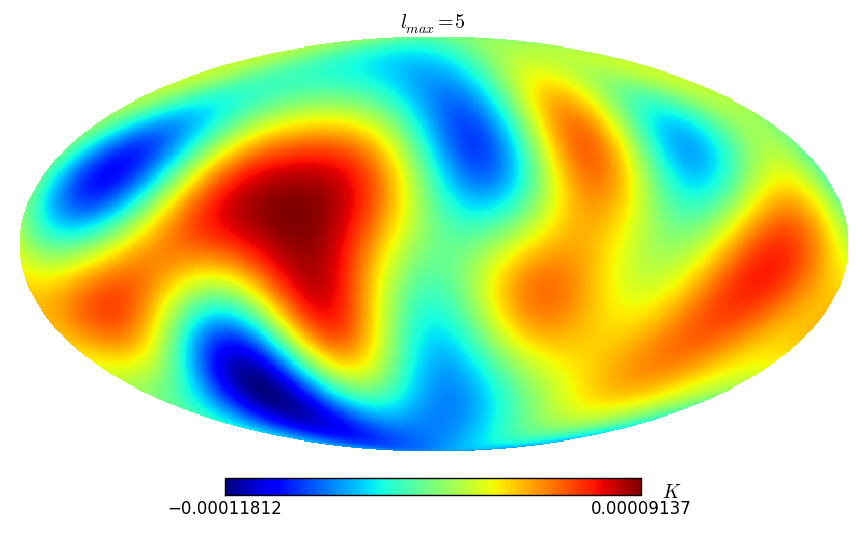
\includegraphics[scale=0.3]{CMB/l5.png}
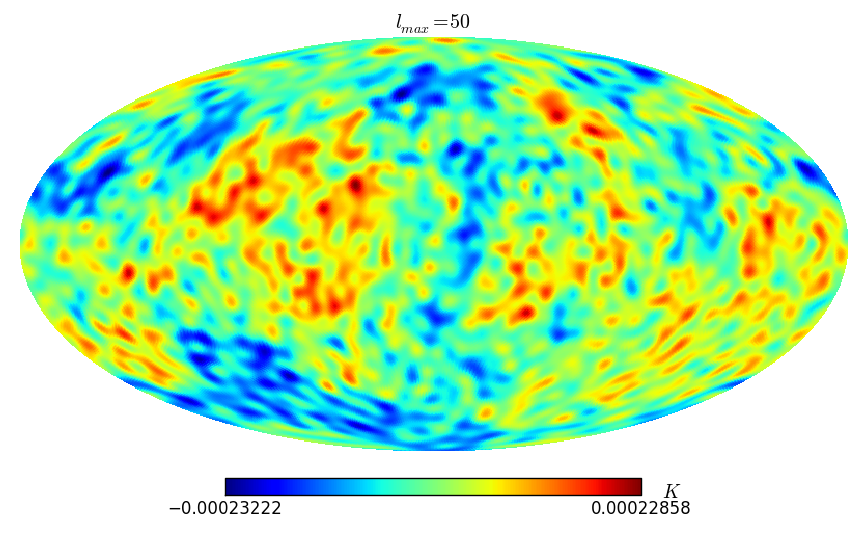
\includegraphics[scale=0.3]{CMB/l50.png}
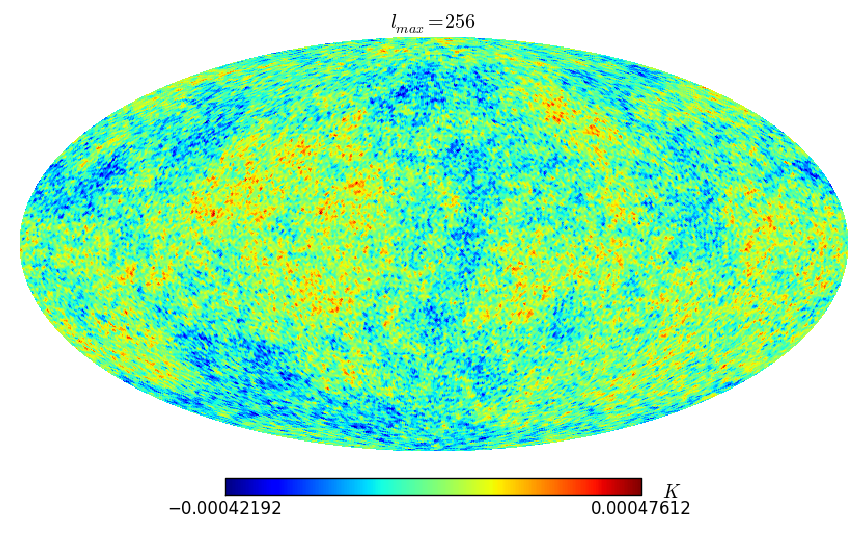
\includegraphics[scale=0.3]{CMB/l256.png}
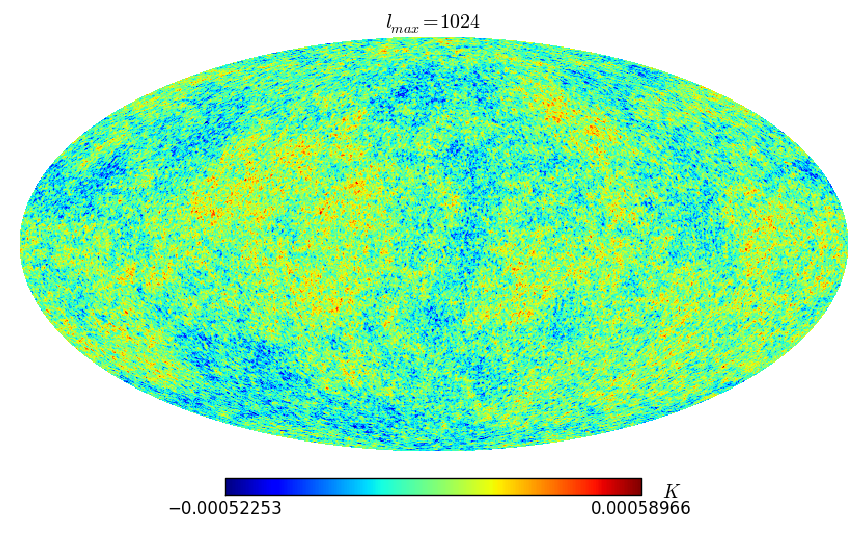
\includegraphics[scale=0.3]{CMB/l1024.png}
\end{center}
\caption{Computer simulated CMB temperature maps including information up to a maximum $l_{max}=5,50,256,1024$, left to right, top to bottom}
\label{simcmbsky}
\end{figure}
\subsection{The CMB anisotropy spectrum}
Now that we have our scale templates for the two dimensional sky, the spherical harmonics $Y_{lm}(\mathbf{\hat{n}})$, we can use them to describe quantitatively the inhomogeneities that we see in Figure \ref{cmbwmap}; a sky map like these contains informations on all angular scales, which means that it will receive the contributions from all the spherical harmonics, and each mode $(l,m)$ will contribute with a coefficient $a_{lm}$. In this picture, giving the values of the measured temperature $T(\mathbf{\hat{n}})$ at every point on the celestial sphere, is equivalent to specifying all the $a_{lm}$ coefficients for $l=0,1,2,...$ and $-l\leq m \leq l$, because we can write the temperature fluctuation $\delta T(\mathbf{\hat{n}})\equiv T(\mathbf{\hat{n}})-T_{CMB}$ as 
\begin{equation}
\delta T(\mathbf{\hat{n}})=\sum_{l=0}^{\infty}\sum_{m=-l}^la_{lm}Y_{lm}(\mathbf{\hat{n}})
\end{equation}
Physically, the coefficients $a$ will depend on the initial conditions that generate the temperature fluctuations at the Big Bang, evolved till the time of recombination. The fact that our universe is statistically isotropical has an important consequence on the coefficients $a_{lm}$: mathematically speaking, for each $l$ the multiplet $(a_{l,-l},...,a_{l,l})$ has special transformation properties, in particular it trasforms as a \textit{spherical tensor} under rotations. Without going into the details, under a rotation, the $m$ components corresponding to the same $l$ will be mixed together with a linear transformation, which however won't mix together different $l$ modes. This means that, if we want to describe a statistically isotropical universe, our $a_{lm}$ coefficients cannot depend on $m$, but on $l$ only! Is that what we observe in a real CMB experiment? Not exactly... To understand why we measure an $m$ dependency in the coefficients we need to understand the concept of \textit{cosmic variance}.   

\subsubsection{The concept of cosmic variance}
%
To get started understanding this concept of cosmic variance, let's start with a simpler example: consider a random number generator, that generates random numbers $x_i$ according to some know probability distribution $p(x)$. It is useful to restrict ourselves to the case where this probability distribution has a Gaussian shape
\begin{equation}
p(x\vert\mu,\sigma)=\frac{1}{\sigma\sqrt{2\pi}}\exp{\left(-\frac{(x-\mu)^2}{2\sigma^2}\right)}
\end{equation} 
%
In this example $\mu$ is called \textit{location parameter}, and gives us an idea on what is the expectation value (or average) of our random draw $x_i$, while $\sigma$ is called \textit{scale parameter} and is a measure of the scatter of our random numbers around the expectation value. Suppose that now we draw $N$ numbers $\{x_i;i=1..N\}$ from our random generator, of which we don't know neither $\mu$ nor $\sigma$: these numbers will be of course different from each other. Given these $N$ numbers we can try to estimate the location parameter $\mu$ and the scale parameter $\sigma$ computing the arithmetic average and the standard deviation of our sample
\begin{equation}
\hat{\mu}=\frac{1}{N}\sum_{i=1}^Nx_i
\end{equation}
\begin{equation}
\hat{\sigma}=\sqrt{\frac{1}{N-1}\sum_{i=1}^N(x_i-\hat{\mu})^2}
\end{equation}
%
Now the question is: when we look at the values $\hat{\mu}$ and $\hat{\sigma}$ that we compute from our sample, will they actually be equal to the true values $\mu$ and $\sigma$? Well in gereral no, because remember that our $x_i$ are random numbers and we have drawn only a finite number $N$ of them. There is a mathematical theorem though, called \textit{central limit theorem}, that says that $\hat{\mu}$ and $\hat{\sigma}$ will differ from the true values only by an amount that decreases with increasing sample size as $1/\sqrt{N}$, i.e. $(\hat{\mu}-\mu)/\mu\propto1/\sqrt{N}$. Now let's go back to our temperature fluctuation coefficients $a_{lm}$. 
Since we believe that these fluctuations were originated by quantum fluctuations of some energy field in the very early universe, we believe that in reality $a_{lm}$s are random numbers drawn from some Gaussian random generator (which in cosmology is called \textit{inflation}). What we see today in the CMB sky is one particular realization of these random numbers; the fact that the universe is statistically isotropical just means that the $a_{lm}$ with the same $l$ are drawn from the \textit{same} Gaussian distribution. 
You may think that, for each fixed $l$, $\{a_{lm}\}$ is a sample of size $N_l=2l+1$ drawn from a Gaussian distribution with location parameter $\mu_l=0$ and scale parameter $\sigma_l=\sqrt{C_l}$. Even if for each $l$ the $a_{lm}$ are drawn from the same distribution, this doesn't mean that they are equal, in the same fashion as the $x_i$, which are drawn from the same distribution but are not equal. The full probability of our CMB sky to be described by a set of coefficients $\{a\}$ is found to be well described by a Gaussian function
\begin{equation}
P(\{a\})\propto \exp{\left(-\sum_{l=0}^\infty\sum_{m=-l}^l\frac{a_{lm}^2}{2C_l}\right)}
\end{equation}
This means that all (or better, almost all, but this is another story...) the statistical information on the universe you can possibly extract from a CMB experiment is stored in the numbers $C_l$, $l=0,1,2,...$, each one carrying information about an angular scale $180^\circ/l$. Since for each $l$ the coefficients $a_{lm}$ are drawn from the same distribution, we can use this sample to estimate a value for the scale parameter $C_l$:
\begin{equation}
\hat{C}_l=\frac{1}{2l+1}\sum_{m=-l}^la^2_{lm}
\end{equation} 
%
This estimate will nail down the measured $\hat{C}_l$ to the true $C_l$ up to a difference that will decrease as $1/2l+1$; this means that the low $l$ modes will be the harder ones to measure, and the ones which will have a larger scatter from the true value! This is the phenomenon called \textit{cosmic variance}. These $C_l$ numbers were actually measured by a variety of different experiments, ground and satellite based, and you can see the results of these measurements in Figure \ref{exppower}
\begin{figure}
\begin{center}
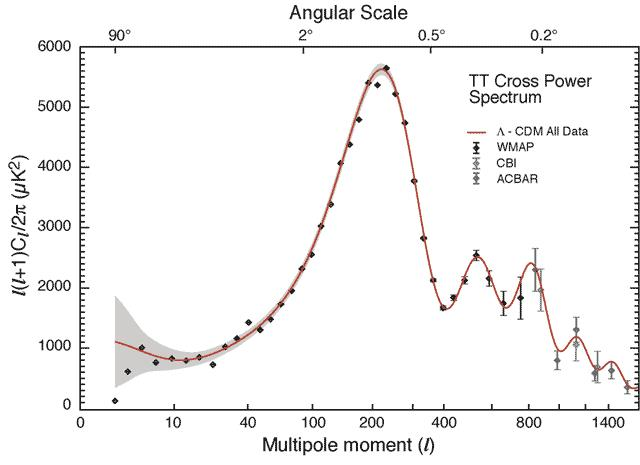
\includegraphics[scale=0.7]{CMB/exp_power}
\label{}
\end{center}
\caption{Experimental \textit{power spectrum} of the CMB (i.e. the set of $C_l$'s) measured by a variety of experiments}
\label{exppower}
\end{figure}
You can immediately see that this spectrum is almost flat for $l\lesssim 100$, which means that the universe is almost isotropical at scales larger than these, peaks at $l\sim 200$ (which corresponds to an angular scale of $\sim 1^\circ$), where the first inhomogeneities start to appear, and then develops an oscillating feature at larger $l$. These oscillations are called \textit{baryonic acoustic oscillations} and contain most of the cosmological information we seek to extract from the CMB. We will outline a physical explanation of these features in the following paragraph. 

\section{The physics behind the CMB anisotropies}
The main purpose of this section is that of giving a physical explanation to the shape of the CMB power spectrum displayed in Figure \ref{exppower}, focusing on the most important and distinctive aspects only. As we can see from a first look, this $C_l$ spectrum exibits a flat shape for low $l$ (large angular scale), which then plummets and peaks at $l\sim 200$ and develops a damped oscillating feature from there on. The first feature we want to understand is the physics that regulates the physics of the first peak.  
\subsection{One degree}
As pointed out several times, the CMB was born when the universe became neutral and electrons and protons recombined, which happened at a time $t_{rec}\approx 300,000\,$yr, or analogously at a redshift $z_{rec}\approx 1000$; let's try to calculate the \textit{size of the horizon} of the universe at this time. This is nothing else than the length a photon, travelling in a straight line at the speed of light, was able to cover from the Big Bang to recombination, which, using equation (\ref{frw}) can be calculated to be
\begin{equation}
l_{hor}=a(t_{rec})\int_0^{t_{rec}}\frac{cdt}{a(t)}=\int_{z_{rec}}^\infty\frac{cdz}{H(z)}
\end{equation} 
A similar reasonment allows us to calculate also $d_A$, which is the \textit{physical distance} that separates us from a light source at redshift $z_{rec}$ (i.e. at the point of origin of the CMB itself), using equation (\ref{distanceredshift})
\begin{equation}
d_A=\int_0^{z_{rec}}\frac{cdz}{H(z)}
\end{equation} 
In our fiducial $\Lambda$CDM model already discussed we have $H(z)=H_0\sqrt{\Omega_\Lambda + \Omega_m(1+z)^3}$ and hence we can calculate the \textit{angular size} $\delta \theta_{hor}$ that the universe's horizon at the time of recombination subtends on the sky today
\begin{equation}
\delta\theta_{hor}=\frac{l_{hor}}{d_A}=\frac{\int_{z_{rec}}^\infty\frac{dz}{\sqrt{\Omega_\Lambda + \Omega_m(1+z)^3}}}{\int_{0}^{z_{rec}}\frac{dz}{\sqrt{\Omega_\Lambda + \Omega_m(1+z)^3}}}
\end{equation}
that, with the numerical values $z_{rec}\approx 1000, \Omega_m\approx 0.25$ and $\Omega_\Lambda\approx 0.75$ results in an angular scale $\delta\theta_{hor}\approx 1^\circ$, which corresponds to the power spectrum in the region $l\sim l_{peak}=180^\circ/\delta\theta_{hor}\approx 200$. The interpretation of the peak now is more clear: any region in the sky that subtends an angular size bigger than $\delta\theta_{hor}$ (and corresponds to the power spectrum region $l\lesssim l_{peak}$) is \textit{causally disconnected} because light, by the time of recombination, didn't have enough time to travel and carry information around it. There will be hence a lack of any kind of information (like temperature fluctuations for example) on scales bigger that one degree, or at $l\lesssim l_{peak}$;  this is qualitatively why the spectrum is flat before $l_{peak}$ and why the first connected cold and hot spots start to appear on angular scales smaller than one degree on the sky. As we will see in the next paragraph, the 
physics of the fluctuation modes on scales smaller than $1^\circ$, or the region of the spectrum with $l>200$, is controlled by very different physical processes than what we examined here. 
\subsection{The acoustic oscillations at $l>200$}
To understand the physical mechanism that regulate the oscillations in the power spectrum in Figure \ref{exppower} we need to develop a little bit of formalism to simplify the description first.
\subsubsection{A little bit of formalism}
We want to introduce a simple physical picture that is able to describe the temperature fluctuations of the universe at the time of recombination; it is these fluctuations, in the end, that will produce the temperature profile that we see in the sky. Let $\bar{T}(t)$ and $\bar{\rho}(t)$ be the average photon temperature and total density of the universe at some time $t$. Since the density and temperature are not homogeneous, but have tiny spatial fluctuations, we introduce these dimensionless quantities that describe the density and temperature differences
\begin{equation}
\delta(\mathbf{x},t)=\frac{\rho(\mathbf{x},t)-\bar{\rho}(t)}{\bar{\rho}(t)}
\end{equation}
\begin{equation}
\Theta(\mathbf{x},t)=\frac{T(\mathbf{x},t)-\bar{T}(t)}{\bar{T}(t)}
\end{equation}
As pointed out in section \ref{fouriersection}, when we have some inhomogeneous quantity it is useful to analyze it in a scale dependent fashon using the Fourier transform tool, except that in this case we have to extend the formalism in three dimensions. For a generic function $f(\mathbf{x})\rightarrow \hat{f}(\mathbf{k})$, where 
$\mathbf{k}=(k_x,k_y,k_z)=\left(\frac{2\pi}{\lambda_x},\frac{2\pi}{\lambda_y},\frac{2\pi}{\lambda_z}\right)$ and $\hat{f}(\mathbf{k})$ contains information on scales $\lambda_x,\lambda_y,\lambda_z$ in the $x,y,z$ directions respectively; in the following we will then use the equivalent fourier transformed quantities $\delta(\mathbf{k},t)$ and $\Theta(\mathbf{k},t)$ instead of the real space ones that depend on $(\mathbf{x},t)$. There is an additional complication: in addition to their energy, photons carry information also about the \textit{direction} they are travelling; this direction can be encoded in a unit vector $\mathbf{\hat{p}}$, that points from the center to a particular point on a surface of a sphere of radius 1, analogously as the unit vector $\mathbf{\hat{n}}$ that we used to describe the temperature fluctuation on the sky $T(\mathbf{\hat{n}})$. In general, the temperature of photons travelling in different directions can be different, and that is why the temperature fluctuation $\Theta(\mathbf{
k},\mathbf{\hat{p}},t)$ must depend on $\mathbf{\hat{p}}$ too; analogously as we did in section \ref{2dsection} with the vector $\mathbf{\hat{n}}$, we switch from the spatial vector $\mathbf{\hat{p}}$ to a couple of integer numbers $(l,m)$ that encode the angular scale information on the temperature variation over different directions. For this particular case, since we will see that all relevant equations for $\Theta$ will depend only on the angle between $\mathbf{\hat{k}}$ and $\mathbf{\hat{p}}$, via the product $\mathbf{\hat{k}}\cdot\mathbf{\hat{p}}$, the only non zero modes in the direction fluctuation of the temperature will be the ones with $m=0$, i.e. the ones with templates $Y_{l,0}(\theta_{\mathbf{\hat{p}}},\phi_{\mathbf{\hat{p}}})\equiv P_l(\mathbf{\hat{k}}\cdot \mathbf{\hat{p}})$. We indicate the $l$th mode of the temperature fluctuation in propagation direction with the notation $\Theta_l$; if you now allow me to use another, more convenient parametrization of time, using the coordinate $\eta$ 
instead of the regular $t$(the two are related by the one to one function $ct(\eta)=\int_0^\eta a(\eta')d\eta'$), we see that we can describe the temperature inhomogeneity of photons, both in space and propagation direction, with the functions $\Theta_l(\mathbf{k},\eta)$. In the next subsection we will see how this description proves to be very useful in describing the evolution of the temperature fluctuations and in particular the state of these fluctuations at recombination. 
\subsubsection{Evolution of inhomogeneities on a rope}
Imagine a rope fixed at two points: if the rope is unperturbed every point $x$ along the rope will be at the equilibrium position $y(x)\equiv0$. This will be the analogous of our uniform universe with $\delta=0$ and $\Theta=0$; now imagine to perturb the rope at some point: this will start an oscillatory behaviour $y(x,\eta)=A(x)\sin{\omega \eta}$ with $A(x)$ some amplitude. This will be the analogous of the temperature and density perturbation evolution with time $\eta$. Now imagine that, while it is oscillating, the rope's extremes are freed at some time $\eta_0$; after this instant, the perturbations in the rope will still evolve, but it will be a free streaming evolution. This will be analogous of what happens after recombination, when the photons stop interacting and free stream to us; the temperature fluctuations, in a sense, will \textit{freeze} at recombination and subsequently evolve in a free streaming fashon. Again, since we are dealing with inhomogeneities, it is better to switch to Fourier modes:
 each perturbation on scale $\lambda=2\pi/k$ (which corresponds to $A(x)=A_0\sin{kx}$ will oscillate with a characteristic frequency $\omega_k=c_s k$, where $c_s$ is the speed of the (''sound'') waves transmitted by the rope. The evolution of the perturbations from the equilibrium position $y(k,\eta)$, on the rope will evolve according to the equation
\begin{equation}
\label{ropewaveeq}
\left(\frac{d^2}{d\eta^2}+\Gamma \frac{d}{d\eta}+\omega_k^2\right)y(k,\eta)=f
\end{equation}
where we introduced the possibility of some friction which dissipates energy along the rope, encoded in the coefficient $\Gamma$, and introduced an \textit{external} constant force $f$ which forces the oscillations. Compare this equation with (\ref{simpleharmonic}); this is just $F=ma$ applied to this system, including the damping $\Gamma$ and the external force. Think about the case $\Gamma=0$ first: suppose that we excite the mode $k$ by an amount $y_0(k)$ at zero time $\eta=0$, and suppose we start from rest $\dot{y_0}(k)=0$. It can be shown that the solution will be in the form 
\begin{equation}
y(k,\eta)=\left(y_0(k)-\frac{f}{\omega_k^2}\right)\cos{\omega_k\eta}+\frac{f}{\omega_k^2}
\end{equation}
and hence this particular $k$ mode will arrive at the point where the rope breaks, at $\eta=\eta_0$, with an amplitude
\begin{equation}
\label{pertfreeze}
y(k,\eta_0)=\left(y_0(k)-\frac{f}{c_s^2k^2}\right)\cos{(c_sk\eta_0)}+\frac{f}{c_s^2k^2}
\end{equation}
After this point the rope will not be bound anymore at its extremes, and the perturbations will be freezed and evolve in a free streaming fashion; if we introduce the damping $\Gamma$ the perturbations will still oscillate, but they will be damped by an exponential factor $e^{-\Gamma \eta/2}$. 
\subsubsection{Evolution of inhomogeneities in the universe}
What does all this rope model have to do with the universe? In fact, a lot: the homogeneous model of the universe is the analogous of our unperturbed, tense rope fixed at the extremes. If we introduce some inhomogeneities in the temperature or density fields (which were generated at very early times during an epoch called \textit{inflation}), as for the rope, these inhomogeneities will start to oscillate. Our displacement $y(k,\eta)$ will become the temperature fluctuation $\Theta_l(\mathbf{k},\eta)$, and the equation which regulates its evolution will no longer be $F=ma$, but the coupled Einstein-Boltzmann differential equations which, under certain approximations, take a suggestive form (at least for the mode with $l=0$)
\begin{equation}
\label{monopolepert}
\left(\frac{d^2}{d\eta^2}+\frac{\dot{R}}{1+R}\frac{d}{d\eta}+\frac{k^2c_s^2}{c^2}\right)[\Theta_0(\mathbf{k},\eta)+\Phi(\mathbf{k},\eta)]=\frac{k^2}{3}\left[\frac{1}{1+R}\Phi -\Psi\right]
\end{equation}  
Ignore the quantities $\Phi,\Psi$, which are some kind of gravitational potentials coming from the Einstein equation, and do not add relevant details to what we are going to say. Just focus on $\theta_0$; this equation is tremendously similar to (\ref{ropewaveeq}), with $\Theta_0$ playing the role of $y$, the right hand side playing the role of the external force and the ratio $\frac{\dot{R}}{1+R}$ playing the role of the damping factor. Here $R=\rho_b/\rho_\gamma$ is the baryon to photon density ratio. The meaning of this term is that, since photons and electrons scatter a lot before recombination, with a mean free path (distance between two interactions) $1/(\sim n_e \sigma_T)\sim 1/(m_e\rho_\gamma R\sigma_T)$, all inhomogeneities with scales smaller than this mean free path will be damped, because the continuous interactions will wash them out really fast. This will introduce a damping factor for all modes with $k\gtrsim k_D=n_e\sigma_T$, analogously to what happens for the damped rope. For the rest, 
analogously as we have seen in the previous paragraph, each oscillation mode $k$ will arrive at recombination with an oscillating amplitude as we have seen in equation (\ref{pertfreeze}) (just substitute $\eta_0\rightarrow \eta_{rec}$) 
\begin{equation}
\label{solmonop}
\Theta_0(\mathbf{k},\eta_{rec})\sim k^{-3/2} \cos{(kc_s\eta_{rec}/c)}e^{-\Gamma(k/k_D)\eta_{rec}}
\end{equation}
where we have encoded the effect of the damping in this $k$ dependent relaxation coefficient $\Gamma$; this discussion is very rough and not very exact, but it allows us to capture the physics underlying these acoustic oscillations that we see in the CMB. The exact solution to equation (\ref{monopolepert}), which allows us to understant with which amplitude each $k$ mode arrives at recombination, is displayed in Figure \ref{kpert} 
\begin{figure}
\begin{center}
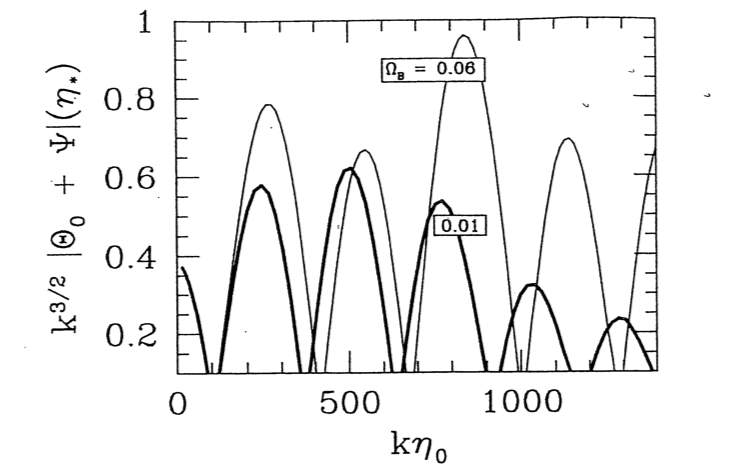
\includegraphics[scale=1.0]{CMB/pert.png}
\end{center}
\caption{Amplitude of each $k$ mode in the temperature fluctuation $\Theta_0$, as it arrives at recombination; the $k^{3/2}$ factor on the vertical axis is there, because each $k$ mode generated at inflation has an initial amplitude (due to quantum mechanical effects) proportional to $k^{-3/2}$. This is the same reason the CMB power spectrum is plotted not as $C_l$ vs $l$, but as $l(l+1)C_l$ vs $l$. Credit for the image: Scott Dodelson, Modern Cosmology ($\eta_*=\eta_{rec}$ in the figure)}
\label{kpert}
\end{figure}
After recombination, these perturbations will be freezed, cause photons do not interact anymore, and will free stream to us; the important point to understand here is that upon free streaming of the perturbations from recombination to us, the different $l$ modes at recombination will mix together to produce a particular $C_l$ we observe today on the sky. This is due to the fact that the CMB temperature profile we observe today on earth is a superposition of all the $\Theta_l$ profiles coming from different positions on the recombination surface (which means coming from different $\mathbf{k}$ values when we switch to Fourier space), as you can see in Figure \ref{convol}.
\begin{figure}
\begin{center}
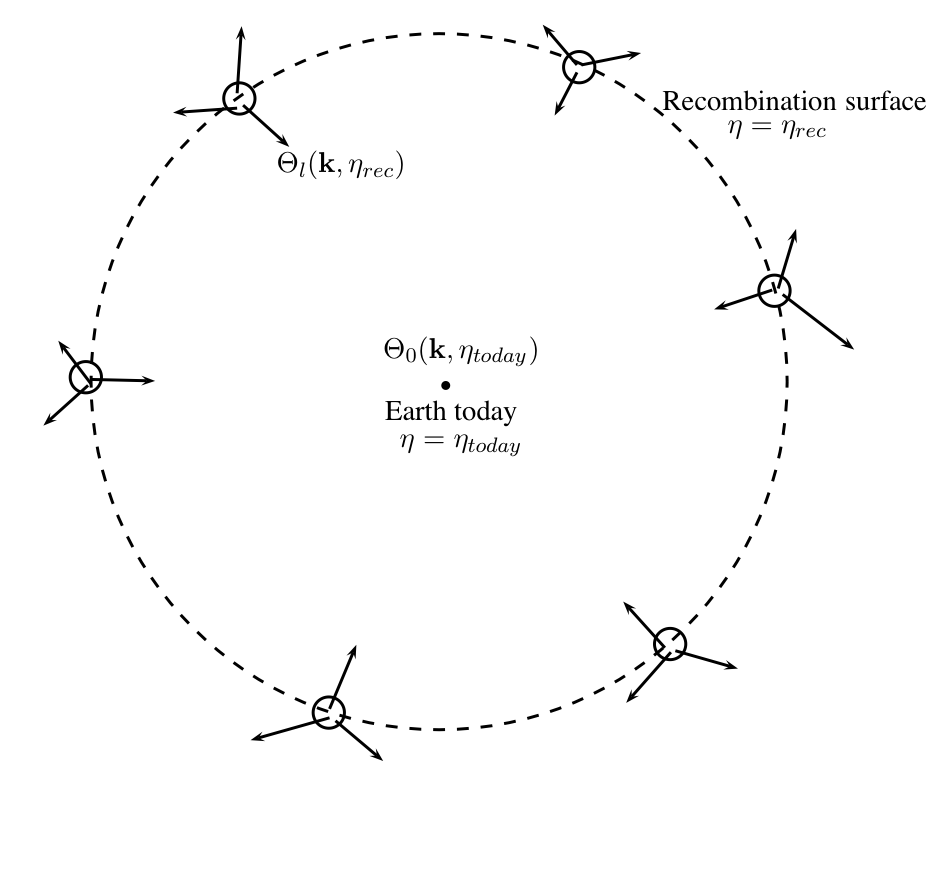
\includegraphics[scale=0.6]{CMB/stream}
\end{center}
\caption{The temperature profile observed today receives contributions from all points on the recombination surface; this means that, when you sum over
$\mathbf{k}$, the different $l$ modes at recombination mix to give a particular mode (for example $l=0$) today. We focus on the contribution of the $l=0$ mode at recombination to the $l$th mode today in equation (\ref{zerotol})}
\label{convol}
\end{figure}
The simplest approximation that makes us understand how this free free streaming mixes $l$ modes, is made observing how the  $l=0$ mode at recombination contributes to the $l$th mode of $\Theta$ observed today. It can be shown that 
\begin{equation}
\label{zerotol}
\Theta_l(\mathbf{k},\eta_{today})\sim[\Theta_0(\mathrm{k},\eta_{rec})+\Psi(\mathbf{k},\eta_{rec})]j_l[k(\eta_{today}-\eta_{rec})]
\end{equation} 
where $j_l(x)$ are special functions that have the behaviour outlined in Figure \ref{bess}. Clearly the $l$th mode of $\Theta$ today will receive contributions also from the higher $\Theta_l$ modes (1,2,...) at recombination, but we neglect this complication for now. 
\begin{figure}
\begin{center}
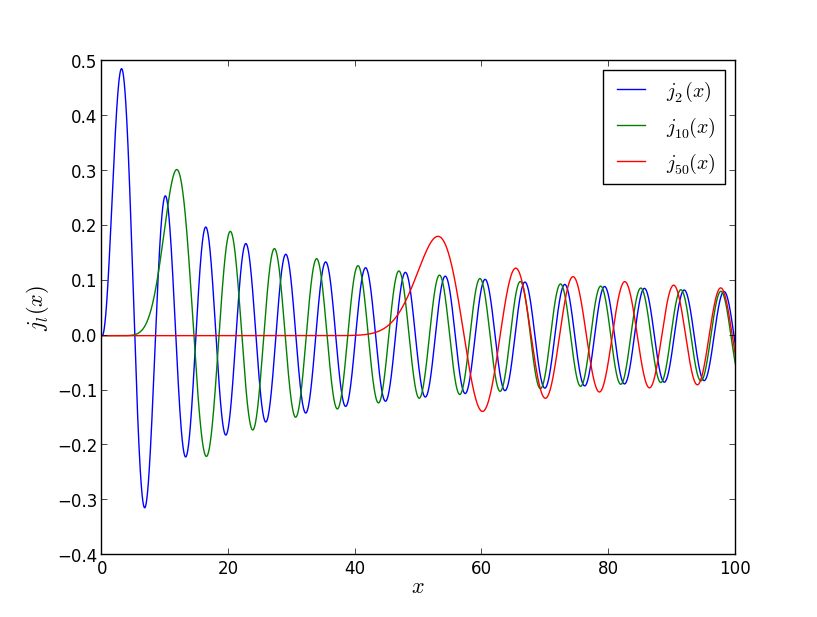
\includegraphics[scale=0.7]{Fourier/bessel.png}
\end{center}
\caption{Behaviour of some of the $j_l$ functions for $l=2,10,50$; you can clearly see that each of these functions has a maximum at $x\approx l$}
\label{bess}
\end{figure}
Since each function $j_l$ peaks at $x\approx l$, we see that $\Theta_l(\mathbf{k},\eta_{today})$ will have its maximum when $k\sim l/\eta_{today}$; since the $C_l$ coefficient are quadratic in the temperature fluctuation, and since the dominant contribution to the $l$th mode of this temperature fluctuation today comes from $\Theta_0(l/\eta_{today},\eta_{rec})$ (this is the mode which is amplified at maximum after free streaming), we immediately see that 
\begin{equation}
C_l\propto \Theta_0^2(k=l/\eta_{today},\eta=\eta_{rec})
\end{equation}
that, along with equation (\ref{solmonop}), gives us a very good explanation of these acoustic oscillations we see in the CMB power spectrum: these oscillations are nothing else that a photograph of the \textit{rope oscillations} that characterized the evolution of the inhomogeneities in the universe's temperature, and froze at recombination. One can do better approximations solving equation (\ref{monopolepert}) exactly, together with the evolution equation for the other modes $\Theta_l$, but this crude approximation we made captures the all the intuitive physics we need to explain this oscillatory damped behaviour we see in the power spectrum. 

\section{Investigating the universe with the CMB}
After all this discussion, what do we learn on the universe from the measurement of these $C_l$ coefficients that we measure in CMB experiments? It might not seem so, but these coefficients are currently the best constraint we have on the universe's energy budget, in terms of dark matter and dark energy. The reason of this is that, as I hope you are aware at this point, all the quantities that determine the location of the acoustic peaks and the shape of the CMB power spectrum, like the speed of sound at recombination $c_s$, or the damping wavenumber $k_D$, strongly depend on the cosmological density parameters (in particular on the baryon density, $\Omega_b$) and on the expansion history of the universe (which is regulated mainly by the dark matter density $\Omega_m$ and by the dark energy density $\Omega_\Lambda$). This dependence is very complicated, and there are no exact formulas to exploit it, so what we usually do is use a public available software, called CAMB, that, given a set of cosmological 
density parameters, solves the Einstein-Boltzmann equations ((\ref{monopolepert}) and the others for $l>0$) and outputs a set of power spectrum coefficients $C_l$ corresponding to the parameters inputed. We then measure which are the actual density parameters of our universe looking at which is the combination results in a simulated power spectrum that matches the experimentally measured one; an example of this is shown in Figure \ref{simpow}.    
\begin{figure}
\begin{center}
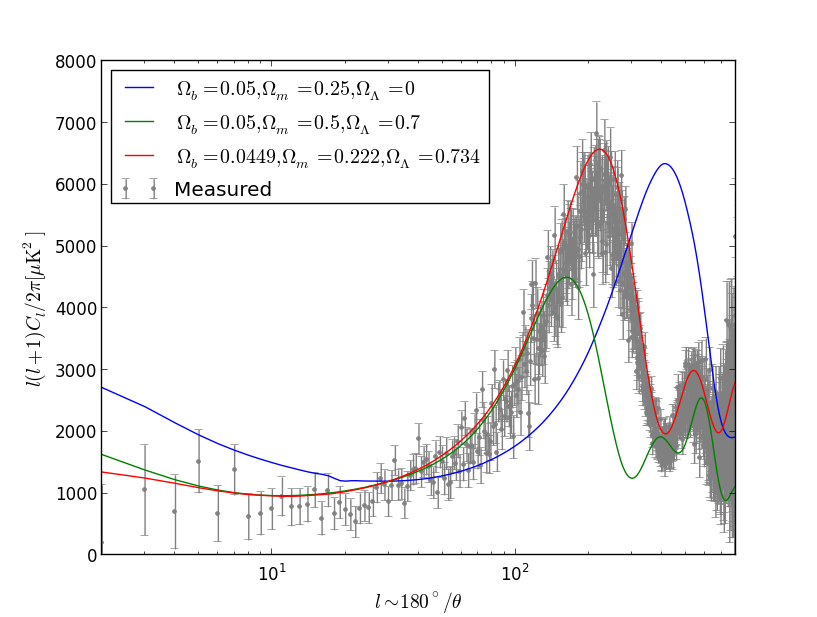
\includegraphics[scale=0.7]{CMB/simulated.png}
\end{center}
\caption{Simulated CMB power spectrum varying the density parameters $\Omega_b,\Omega_m,\Omega_\Lambda$; only one of the three combinations tried, correctly predicts the location of the acoustic peaks}
\label{simpow}
\end{figure}
You can clearly see from this plot that our observations strongly indicate a scenario in which ordinary matter (baryons) make up for $5\%$ of the energy budget, $22\%$ is dark matter and $73\%$ is made up by dark energy. This method can be used to constrain also other parameters, like the Hubble parameter today, $H_0$, and the amplitude of density fluctuations on a coventional scale of 8\,Mpc, $\sigma_8$.